	\section{Motivation and objectives}
	
	To these days, and since long time ago financists, economists, statisticians tried to figure out an exact method 
	to predict the fluctuations of the price based mostly on its history. This methods are quiet accurate in ideal
	conditions; if we remember the financial crisis that happen in the 2008 (For more details about the crisis there 
	are two brief and concrete articles \cite[section: abstract \& origins]{R2010} \cite[p. 1-3]{P2009}), this is not a normal situation of any 
	market. And of course predictions said something while the actual numbers where not reflecting the previous
	forecasts. 
	
	The aim of this thesis is not to develop a new method in order to predict the price or to tell an investor to buy
	or not to buy a particular stock, but to realize how qualitative aspects (what is written on the news) could be 
	correlated with the price changes of a stock.
	
	Initially we will assume the most natural position: That the positive news are positively correlated with the 
	positive increments of the stock and vice-versa: the negative news are positively correlated with the drops
	in the stock prices.
	
	Before we will go deep, we will answer several questions to clarify some technical terms non-computer science
	related. And for this we will rely on several literature.
	
	%\cite[p. 2]{D2011}
	
	\begin{itemize}
		\item How a market works? \\
		According to Patel \cite[p. 24]{P2007}: \\ \emph{"Any market is made of buyers and sellers/suppliers and there is always a conflict going on between these two groups. Buyers want to pay the minimum possible price while sellers on the other hand want to get maximum possible price. If the price is too low, buyers would demand a large quantity but sellers would not want to sell much at this low price. If price is too high, sellers would love to sell a large quantity but buyers would not want to buy much. This is a kind of war between two groups - one trying to push prices lower and the other one trying to push prices higher. In market economy, price keeps changing until it reaches a point where the quantity demanded by buyers equals quantity supplied by sellers."}
		
		\item Why stock prices changes?\\
		According to Patel \cite[p. 24]{P2007}, \\ \emph{"One will see these Demand and Supply curves change more rapidly for a stock than for any other item. That is why we see stock prices changing almost every moment. For a stock, individuals and institutions that hold the stock or intend to short the stock are the potential sellers and they collectively define the supply curve. There are thousands, if not millions, of reasons that may motivate or prompt a market participant to sell a particular stock he or she is holding or intending to short sell. Similarly, individuals and institutions that are thinking/planning to buy the stock form the Demand curve. There would also be several reasons why they want to buy this stock. As we all know, a stock’s price is likely to go up if the Demand is increasing or the Supply is decreasing. Similarly it is no rocket science to figure out that a stock’s price would drop if the Demand is shrinking and/or the Supply is expanding. So when a trader is buying a stock, he wants its prices to go up after he has bought it. He wants the Demand for the stock to go up or the supply to dry up."}
		
		\item How often stock prices changes?
		According to Patel \cite[p. 24,25]{P2007}, \\ \emph{"The demand and supply curves for any stock are constantly changing. Variety of economy, industry related or company related events, news, discussions, analyst reports and political and global developments constantly change the demand and supply curves for any stock. Add to this, the fact that given a certain piece of information, a person can’t be sure how people will react to it. Aren’t you surprised to see that even after some unexpected strong positive news about a stock, the stock keeps being traded! Ideally, if the news is too good, everybody should be a buyer and there should be no seller! If there were no seller, there would be no trade! But the fact that most of the stocks keep trading every moment when the Market is open indicates just one thing: There are people with totally different views about the prospects of a stock at any given moment. Everyone who is driven to buy or sell a stock has his own criteria to value the stock, his own set of expectations, and his own unique financial situations and circumstances. This makes it almost impossible to draw complete demand and supply curve for any stock at any point in time."}
		
		\item What does the stock price represents?
		According to Patel \cite[p. 25]{P2007}, \\ \emph{"The net impact of everything happening in a stock or a company gets immediately reflected in the price of the stock. Price is the point where millions of different counter acting forces balance out. So with enough attention to changes in the price of a stock over a day or two, there will be times when we can visualize changes that are taking place in aggregate demand/supply of that stock, and based on that, we will be able to determine in which direction the price of the stock is likely to move over the next few days. There is no need to get into complex world of demand and supply curves; all we need is to keep an eye on where the balance between them is heading."}
	\end{itemize}

	\section{Problem statement}
	
	The main sight of this thesis is to  provide a \emph{Framework} to retrieve, analyze and summarize data from news articles in order to provide qualitative information about some particular company.  

	\section{State of the Art}
	
	The main goal of our project is to consider not only quantitative (stock price of a company, ratios, etc.) factors about the stock market, but to consider the qualitative part (News articles mostly) in order to analyze what is the trends of this qualitative aspects.

	And to perform this analysis we will use several techniques and algorithms (Web crawlers and Sentiment Analysis), and we will be mentioning the highest level of development of this techniques until today. We will help ourselves with some part of a thesis written by Avni Gural \cite{V2013}, in order to describe the state of the art of our techniques and algorithms.
	
	\subsection{Web Crawlers}
	
	We will describe the state of the art of Web Crawlers, according to Gural \cite{V2013}
	\\ A web crawler, also known as harvester, spider, or robot, is an application that browses the World Wide Web and automatically downloads web pages and also can be used for gathering specific information, like in our case; news articles. The main part of such a basic crawler is the download queue, (or sometimes referred as frontier). The most important property for a crawler is the speed. A specialized version of crawling, called focused web crawling, is proposed aiming to collect on-topic data which actually reduces the search space.
			
	Web crawling has many challenges. As stated by Najork \cite[p. 3462-3465]{N2009}, all challenges are ultimately related to scale in deed. A typical crawler has to fetch thousands of pages in a second in order to maintain a fresh corpus of search engine with a couple of billion pages. We can observe in the figure \ref{fig:Crawler_001} the basic architecture of a web crawler.
	
	\begin{figure}\centering
		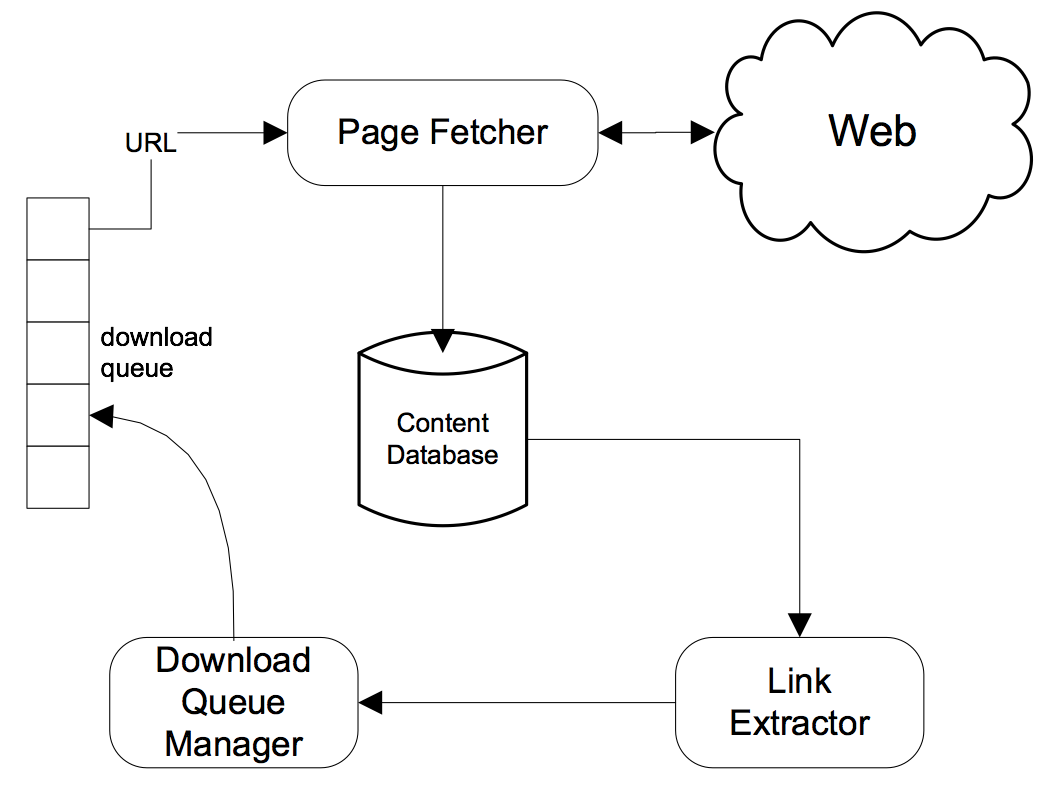
\includegraphics[scale=0.3]{Crawler_001}
		\caption{Basic web crawler algorithm.}\label{fig:Crawler_001}
	\end{figure}
		
	\begin{itemize}
		\item Content Selection: Crawlers should bypass irrelevant, low-quality, malicious content.
		\item Scale: Web hosts an enormous amount of data but the crawlers seek broad coverage and freshness.
		\item Speed: The basic and fast way of keeping track of visited URLs is storing in the memory. However, it is not possible to store hundreds of millions of URLs in the memory. That is why such lists are kept on disk, but accessing nd re-ordering the list becomes slower which degrades the crawling performance.
		\item Infrastructure Cost: According to a blog post on the Official Google Blog \cite{A2013}, the Google index now contains about 1 trillion unique URL's. This graph of one trillion URLs is similar to a map made up of one trillion intersections, which is continuously reprocessed several times per day. Storing, indexing and fresh-keeping such a huge data requires massive investments on hardware infrastructure.
		\item Ethics / Politeness: Crawlers should prevent server overload and comply with Robot Exclusion Protocol (which is a de facto standard for definition of access rights on a website for crawling) \cite{K2013}.
	\end{itemize}
	
	\subsubsection{Focused Web Crawling}\label{focusedWebCrawling}

	One of the most important properties for a crawler is the speed. The web, hosting an enormous amount of data in various forms, is estimated to have more than 10 billion pages and continues to grow rapidly \cite{WWW2013}. Crawlers should discover and use not only the new pages but also the recent versions of the pages. A general purpose crawler is said to be neither necessary nor sufficient to crawl and index such a giant amount of web pages. Therefore, a specialized version of crawling, called focused web crawling, is proposed aiming to collect on-topic data which actually reduces the search space.
	
	The first related work on focused crawling was done by De Bra et al. \cite[p. 481-493]{B1994}, called fish search. In this research, for a client-based search engine, a simulated group of fish crawls on the web and assigns page relevance metric to pages using a binary classification with an input of simple keyword or regular expression. The lifespan of a fish depends on visited page relevance, where the fish dies when a specified amount of irrelevant pages are traversed. In addition, a fish produces offspring when a new page is traversed. Fish search works as depth-first search, since new URLs are added to the beginning of the download queue.
	
	Later, an extended version of fish search was developed, so called shark search, it was proposed by Hersovici et al. \cite[p. 317-326]{H1998}. In contrast to fish search, shark search estimates page relevance with a continuous function resulting a real number between 0 and 1 for the a similarity between document and query. Then, in the download queue, URLs are ordered by linear combination of source page relevance, anchor text and neighborhood of the link on the source page.

	\subsection{Sentiment Analysis}
	
	Opinions as the key influencers of our behavior are important. As Liu stated in \cite{L2011}, our beliefs and perceptions of the reality, and the choices we make, are susceptible on how others see and evaluate the world. This is the reason why people seek out opinions of others when making a decision. Sentiment analysis (a.k.a. opinion mining) is an area of study and analyzing people's opinions, appraisals, attitudes, feelings, and emotions toward entities, individuals, issues, events, topics, and their attributes. Sentiment analysis has been an active research area for quite some time. Feldman in \cite[p. 82-89]{F2013} states that there are over 7,000 articles on the topic of sentiment analysis.
	
	\begin{figure}\centering
		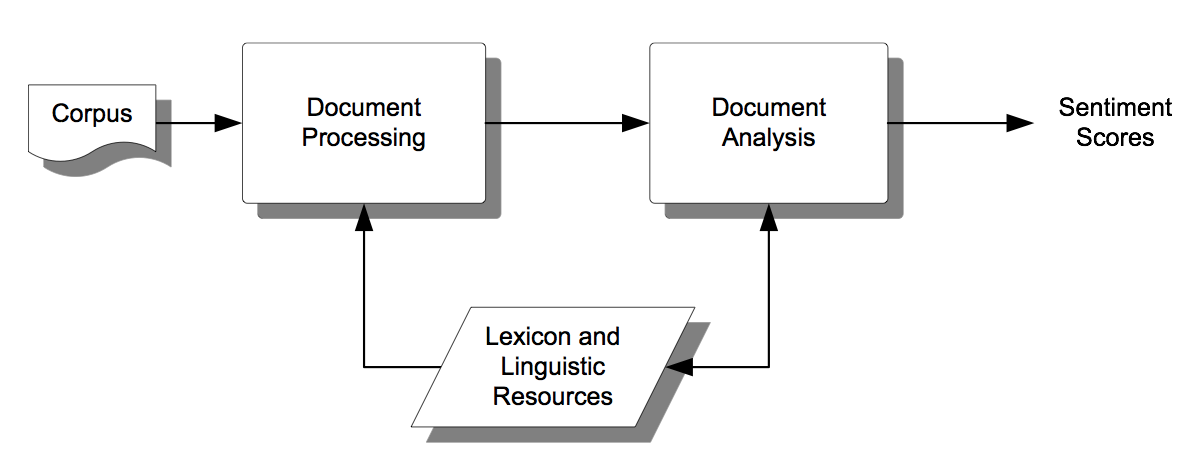
\includegraphics[scale=0.3]{Sentiment_001}
		\caption{The pipeline of modules in a generic sentiment analysis framework.}\label{fig:Sentiment_001}
	\end{figure}
	
	As Feldman stated in \cite{F2013}, apart from the techniques applied, all sentiment analysis systems implement a generic pipeline, which is illustrated in Figure \ref{fig:Sentiment_001}. The input for a sentiment analysis framework is a corpus of documents, which may include a web page, news articles (which is particularly our case) a short post, or a text document in any format. The corpus is pre-processed by document processing module, which converts corpus to texts by using linguistic resources for stemming, tokenization etc. Then pre-processed texts are sent to the document analysis module which annotates them using the linguistic resources and sometimes with a dictionary of words, called lexicon, which includes annotations of word's sentiment strength. The primary source of subjective content in a textual content can be adjectives (\cite{H1997}, \cite{H2004}); adverbs \cite{B2007} ; adjectives and verbs \cite{K2004}; or exclusive use of verbs \cite{S2008}. The output of the framework is the annotations which can be attached to whole document, to sentences, to entities as sentiment scores.
	
	The document analysis module, which is the main module of the framework, can apply two main lines of techniques for annotation: machine-learned and lexicon-based. In machine-learned sentiment analysis techniques \cite{P2002}, a model is built by a training dataset using common machine learning algorithms such as SVM, Naive Bayes, Logistics Regression, or KNN. Each document instance (e.g., a product review) in the dataset is associated with a value indicating the strength and polarity of the sentiments expressed in the text. In practice, obtaining large-scale labeled datasets is difficult, and the existing datasets are often domain-specific. As a remedy, the lexicon-based sentiment analysis techniques (\cite{B2010}, \cite{T2010}, \cite{TB2011}) aim to create a vocabulary and a set of rules to quantify the amount of sentiments in a given piece of text, eliminating the dependency to labeled training data. The vocabulary and rules are created by manually, or expanded by utilizing resources like WordNet \cite{M1995}.
	
		
	\section{General overview}
	
\begin{algorithm}
\caption{General Algorithm}\label{generalAlgorithm}
\begin{algorithmic}[1]
\FOR {\text{each company}}
	\STATE \text{Crawl News articles;}
	\STATE \text{Extract} \textit{article: date, title, content, author}\text{;}
	\STATE \text{Classify} \textit{article}\text{;}
	\STATE \text{Save} \textit{article}\text{;}
\ENDFOR
\STATE \text{Summarize} \textit{articles}\text{;}
\STATE \text{Download \& Save} \textit{stock prices}\text{;}
\end{algorithmic}
\end{algorithm}

Each part of the algorithm \ref{generalAlgorithm} basically will take one or several sections in this work. This general algorithm is the highest level of abstraction of this work, and it will be repeating the process for each of the predefined companies (see the table \ref{tab:analyzedCompanies}). For each company, we will crawl the news for this company (as shown in section \ref{newsCrawler}), then we will extract the information of our interest (as described in section \ref{locators}), after this we will classify the article in positive or negative (according to the section \ref{sentimentAnalysis}), finally we will be saving every article in our page repository \ref{pageRepository}. When we will finish the iteration for all companies we will summarize the data and download the stock prices as described in the section \ref{priceRetrieval}.
	
	
% 	There are two basic ways in the world of dictionary word-based algorithms. The both of them are based on dictionary method \gls{LZW}. The method Word-Based \gls{LZW}, independently presented by Horspool and Cormack \cite{HC92}, and Jiang and Jones \cite{JJ92} in 1992 as first, is adaptive version of mentioned algorithm. The main sight is recently concentred to word-based context methods of data compression and related word-based \textit{preprocessing} transformations, which reversibly transform a data into another form. The reverse process is called \textit{postprocessing} transformation. Affected data could be compressed with most of existing lossless data compression algorithms with better compression efficiency than it can be achieved using an unaltered data. 